\documentclass[letterpaper,11pt]{article}
\pdfoutput=1

\usepackage[margin=2cm]{geometry}
\usepackage{graphicx}

\begin{document}

\begin{figure}
  \centering
  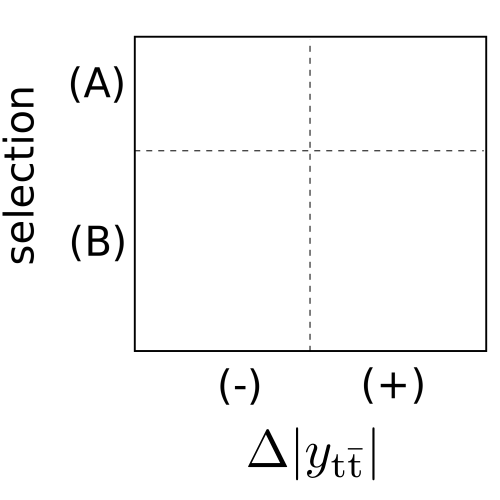
\includegraphics[width=0.3\linewidth]{axes}
  \caption{\label{axes} Four bins, selected (A) and unselected (B) on
    the selection axis, and $(-)$ and $(+)$ on the axis of the the
    observable for which the asymmetry is of interest.}
\end{figure}

\section{Demonstration of technique failures}

Consider a two dimensional distribution of four bins, where one axis
is a selection observable with bins (selected, A) and (unselected, B),
and the other is an observable for which the asymmetry is of interest,
for example $\Delta|y_{\mathrm{t\bar{t}}}|$, with bins $(+)$ and
$(-)$.  Figure \ref{axes} shows the axes. In a model $N$, the
selection contains $N_A$ events and has asymmetry $\alpha_A$, while
the unselected events number $N_B$ and may have a different asymmetry
$\alpha_B$.  The counts in each bin of the model are given by
\[N_x^{\pm} = N_x(1\pm\alpha_x)/2,\]
where $N_x=N_x^-+N_x^+$, and the total asymmetry is given by
\[\alpha = \frac{N_A\alpha_A + N_B\alpha_B}{N_A+N_B}.\]
Note that $\alpha_A\ne\alpha_B$ if and only if the selection
efficiencies for the bins $(+)$ and $(-)$ are unequal.

Suppose we want to measure the asymmetry of an alternative model $D$
which has an antisymmetric component proportional to that of model
$N$, with factor $F$,
\[D_x^{\pm} = N_x(1\pm F\alpha_x)/2,\]
and where we suppose that $D_x=N_x$.  The total asymmetry in model $D$
would be $F\alpha$.


\subsection{Template Strategy}
Following the template strategy we have so far employed, the weights
which symmetrize and antisymmetrize the original distribution after
integrating over the selection axis would be
\[W^\pm_{\mathrm{symm}} = (1\pm\alpha)^{-1},\]
\[W^\pm_{\mathrm{anti}} = \pm\alpha(1\pm\alpha)^{-1}.\]
The templates for the selection would be
\[T^{\pm}_{\mathrm{symm}} = \frac{N_A}{2}\frac{1\pm\alpha_A}{1\pm\alpha},\]
\[T^{\pm}_{\mathrm{anti}} = \pm\alpha\frac{N_A}{2}\frac{1\pm\alpha_A}{1\pm\alpha},\]
and the parametrized template model would be
\[T^{\pm}(f) = T^{\pm}_{\mathrm{symm}} + f\cdot T^\pm_{\mathrm{anti}} = \frac{N_A}{2}\frac{1\pm\alpha_A}{1\pm\alpha}(1\pm f\cdot\alpha).\]
Our expectation has been that $T^\pm(f) = D^\pm_A$ when $f=F$, but
that is clearly only the case if $F=f=1$ or $\alpha=\alpha_A$.  The
former condition is useless for a measurement, while the latter
condition is generally unmet, and is particularly untrue in the cases
of our subselections at extremes of $\mathrm{t\bar{t}}$ system
rapidity and mass.

\subsection{Unfolding Strategy}
The ratios $R_N^{\pm}=N^{\pm}_A/N^{\pm}_B$ given by the model are used
to calculate the corresponding unselected bins
\[U^{\pm}_B = D^{\pm}_A/R^\pm_N = D^\pm_B\left(\frac{1\pm\alpha_A}{1\pm\alpha_B}\right)\]
The expectation that $U^\pm_B=D^\pm_B$ is not met, leading to a
mistake in calculating a corresponding total asymmetry
\begin{eqnarray*}
  \alpha' &=& \frac{D^+_A+U^+_B - D^-_A -
    U^-_B}{D^+_A+U^+_A+D^-_A+U^-_B}\\
  %&=& F \cdot \left(\frac{N_A\alpha_A + N_B\left[\alpha_A\left(\frac{1-\alpha_A\alpha_B}{1-\alpha_A^2}\right) + \frac{1}{F}\left(\frac{\alpha_B-\alpha_A}{1-\alpha_A^2}\right)\right]}{N_A+N_B\left[\left(\frac{1-\alpha_A\alpha_B}{1-\alpha_A^2}\right)+F\alpha_A\left(\frac{\alpha_B-\alpha_A}{1-\alpha_A^2}\right)\right]}\right)\\
  &=& F \alpha_A\cdot \left(\frac{N_A/N_B + \left[(1-\alpha_A\alpha_B) + \left(\frac{\alpha_B}{\alpha_A}-1\right)/F\right]/(1-\alpha_A^2)}{N_A/N_B+\left[\left(1-\alpha_A\alpha_B\right)+F\alpha_A\left(\alpha_B-\alpha_A\right)\right]/(1-\alpha_A^2)}\right)
\end{eqnarray*}
As an example of the significant measurement errors which can be
introduced by this flawed calculation, consider the plausible case
$\alpha_A=0\ne\alpha_B$.  We would find $\alpha' = \alpha \ne F\alpha$.

In the {\sc POWHEG} $\mathrm{t\bar{t}}$ simulation of CMS events
(model $N$, suppose), we have $\alpha=A_c^y\approx0.0056$, a selection
efficiency in lepton+jets channels of $N_A/(N_A+N_B)\approx 0.05$,
$\alpha_A\approx0.0032$, which implies $\alpha_B\approx0.0057$ and
$N_A/N_B\approx0.052$.  The true asymmetry in model $D$, given by
$F\alpha$, and the asymmetry $\alpha'$ calculated by unfolding model
$D$ using ratios $R_N^\pm$, are plotted in Figure \ref{plot} as a
function of the scale factor $F$.  We see that $\alpha'$ and $F\alpha$
have very different slopes as a function of $F$, and coincide only for
$F=1$, when models $N$ and $D$ coincide.
\begin{figure}
  \centering
  \includegraphics[width=0.5\textwidth]{plot}
  \caption{\label{plot} Modeled $A_c^y$ and its calculation from a CMS
    lepton+jets subselection via unfolding, as a function of the
    amplitude $F$ of the {\sc POWHEG} antisymmetric component.  Only
    when $F=1$ does the unfolding procedure yield the correct result.}
\end{figure}

The behavior presented here is not identified in the various analyses
using the unfolding technique because they do not use models of the
form $D_x^\pm$ for ensemble testing cross-checks of the technique.
Rather than scaling the antisymmetric component of the simulation to
construct alternative models, they reweight events with weights
linearly dependent on the value of the observable of interest.  To
demonstrate properties of this construction with our four-bin example,
it is sufficient to assume uniform distribution of events within each
bin, and a differential weight factor $k$.  The models constructed for
ensemble testing cross-checks by analyses using the unfolding
technique are
\[E_x^\pm = \frac{N_x}{2}(1\pm\alpha_x)(1\pm k) = \frac{N_x}{2}(1+k\alpha_x\pm(k+\alpha_x)),\]
which have selected and unselected asymmetries
\[\alpha^E_x = \frac{\alpha_x+k}{1+k\alpha_x},\]
selected and unselected event counts
\[E_x = N_x(1+k\alpha_x),\]
and total asymmetry
\[\alpha^E = \frac{\alpha_A+\alpha_B+2k}{N_A(1+k\alpha_A)+N_B(1+k\alpha_B)}.\]
Appropriately scaling model $E$ to get the correct total event counts,
with a factor $(N_A+N_B)/(N_A(1+k\alpha_A)+N_B(1+k\alpha_B))$, is not
a problem.  The important property of models $E$ is that the ratios of
selected to unselected events are identical to those of model $N$,
since the weight factor cancels in the ratio,
\[R^\pm_N = R^\pm_E \ne R^\pm_D.\]
Therefore, using $R^\pm_N$ in the unfolding procedure for models $E$
yeilds the expected asymmetry $\alpha^E$, although it did not for
models $D$.

The question we must resolve, it seems, is whether models $D$ or $E$
are more likely descriptions of nature.  The idea (model $D$) that the
differential cross sections produced by our generators have correctly
shaped antisymmetric components is incompatible with the idea (model
$E$) that the generators and simulation correctly model the selection
efficiencies.  To me, the latter is more intuitive.

\section{Successful techniques}

\subsection{Alternative Template Strategy}

Rather than using weights to construct templates, we can use the
symmetrized and antisymmetrized components of the selected events.
The statistical power of the templates is reduced compared to the
reweighting strategy, but this alternative does not require
$\alpha_A=\alpha_B$.  The symmetric and antisymmetric components of
the selected events are
\[T^\pm_{\mathrm{symm}} = \frac{N_A}{2}, \qquad T^\pm_{\mathrm{anti}} = \pm\alpha_A\frac{N_A}{2}\]
Using these as templates with a factor $f$ on the antisymmetric
component results in
\[T^\pm(f) = T^\pm_{\mathrm{symm}} + f\cdot T^\pm_{\mathrm{anti}} = N_A(1\pm f\alpha_A)/2\]
As we expect, $T^\pm(f)=D^\pm_A$ when $f=F$.  This technique
generalizes to an arbitrary number of bins in the asymmetry
observable.

\subsection{Reconstruction effects}

Suppose our 

\end{document}
